\PassOptionsToPackage{usenames,dvipsnames}{xcolor}
\documentclass[tikz,border=2]{standalone}
\usetikzlibrary{shadows,arrows,shapes,positioning,calc,backgrounds,fit}
% Define the layers to draw the diagram
%
\begin{document}
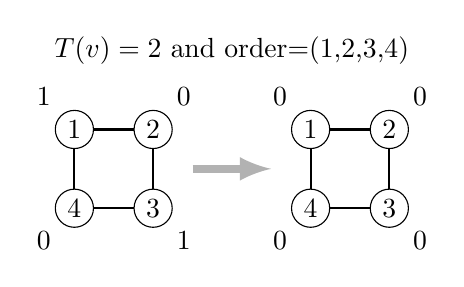
\begin{tikzpicture}
[node distance=1cm,
vertex/.style={shape=circle,draw=black,inner sep=2pt},
thickedge/.style={draw=Gray!60,>=latex, shorten >=.0pt, shorten <=.0pt, 
line width=1mm},
myedge/.style={thick}]
%%
\node (v1) [vertex,label=below left:$0$] at (0,0) {$4$};
\node (v2) [vertex,right of=v1,label=below right:$1$] {$3$};
\node (v3) [vertex,above of=v2,label=above right:$0$] {$2$};
\node (v4) [vertex,above of=v1,label=above left:$1$] {$1$};
\draw[myedge] (v1) -- (v2) -- (v3) -- (v4) -- (v1);
\node at (2,2) {$T(v)=2$ and order=(1,2,3,4)};
%%
\draw[thickedge,->] (1.5,0.5) -- (2.5,0.5);
%%
\begin{scope}[shift={(3,0)}]
\node (v1) [vertex,label=below left:$0$] at (0,0) {$4$};
\node (v2) [vertex,right of=v1,label=below right:$0$] {$3$};
\node (v3) [vertex,above of=v2,label=above right:$0$] {$2$};
\node (v4) [vertex,above of=v1,label=above left:$0$] {$1$};
\draw[myedge] (v1) -- (v2) -- (v3) -- (v4) -- (v1);
\end{scope}
\end{tikzpicture}
\end{document}
